\chapter{Multi-objective optimization}
\label{chapter:metaheuristcs}
\index{Multi-objective optimization}

In this chapter, we focus on establishing the principles about the optimization algorithms that are used to tackle the problems that are going to be used to solve the molecular docking problem. We start from a classic optimization approach to define the concept of metaheuristic and to understand its classification. Then, multi-objective optimization concepts are introduced, as we are dealing with molecular docking problems where the components of the energy function can be optimized at the same time. Finally, we end the chapter with the statistic procedure that has been followed to evaluate the different metaheuristics, where the main performance measures are introduced, as well as the quality indicators that have been used in single-objective and multi-objective optimization problems.

\section{Definition}

Optimization in the sense of finding the best solution, or at least a good enough solution, for a problem is a  vital importance field in the real world and, particularly, in molecular docking. We are constantly solving optimization problems, as searching the shortest path to go from some place to another, organizing our activity schedule, etc. Generally, these problems are small enough, so it is possible to solve them by ourselves without additional help. However, as these problems get larger and more complex, computer assistance is inevitable to solve them.

We start giving a formal definition about the concept of optimization. Assuming, without loss of generality, the minimization case, we can define an \emph{optimization problem}\index{Optimization problem} as follows:

\begin{definition}[Optimization problem]
	\label{def:OptimizationProblem} An optimization problem is formalized as a pair $(S,f)$, where $S\neq \emptyset$ represents the solution space (or search space) of the problem, while $f$ is a function named \emph{objective function}\index{Objective function} or \emph{fitness function}\index{Fitness function}, that is defined as:
	\begin{equation}
		f:S\rightarrow \mathbb{R} \enspace .
	\end{equation}
	Therefore, solving an optimization problem consists in finding a solution, $i^\ast \in S$, that satisfies the following inequality:
	\begin{equation}
	f(i^\ast) \leq f(i), \enspace \enspace \enspace \forall \;\; i\in S \enspace.
	\end{equation}
\end{definition}

Assuming the case of maximization or minimization does not restrict the generality of the results, as it is possible to establish an equality between maximization and minimization problems as follows~\cite{baeck96evolutionary,goldberg89genetic}:

\begin{equation}
\max \{f(i) | i \in S \} \equiv \min \{-f(i) | i \in S \} \enspace. \vspace{0.3cm}
\end{equation}

Depending on the domain to which $S$ belongs, we can define \emph{binary}\index{Binary optimization problem} ($S\subseteq \mathbb{B}^\ast$), \emph{integer}\index{Integer optimization problem} ($S\subseteq \mathbb{N}^\ast$), \emph{continuous}\index{Continuous optimization problem} ($S\subseteq \mathbb{R}^\ast$),
or \emph{heterogeneous}\index{Heterogeneous optimization problem} ($S\subseteq (\mathbb{B} \cup \mathbb{N} \cup
\mathbb{R})^\ast$) optimization problems.

Due to the great importance of the optimization problems, throughout the history of computing, several methods have been developed to try solving them. A very simple classification of these methods is shown in the Figure~\ref{fig:OptTechClass}. Initially, the techniques can be classified as exact (or enumerative, exhaustive, etc.) and approximate. Exact techniques\index{Exact optimization techniques} guarantee to find the optimal solution from any problem instance in a bounded time. The disadvantage of these methods is that the time and / or memory needed, although bounded, grow exponentially with the size of the problem, as most of them are NP-hard. This means in many cases that the use of these techniques is not feasible, since much time  (possibly thousands of years) and / or an exorbitant amount of memory for the problem is required. For these reasons, approximate algorithms\index{Approximate optimization techniques} to solve these problems are receiving increasing attention from the international community for some decades. These methods sacrifice the guarantee of finding the optimum in exchange for finding a satisfactory solution in a reasonable time.

\begin{figure}[H] %tb
	\vspace{0.5cm} \centering 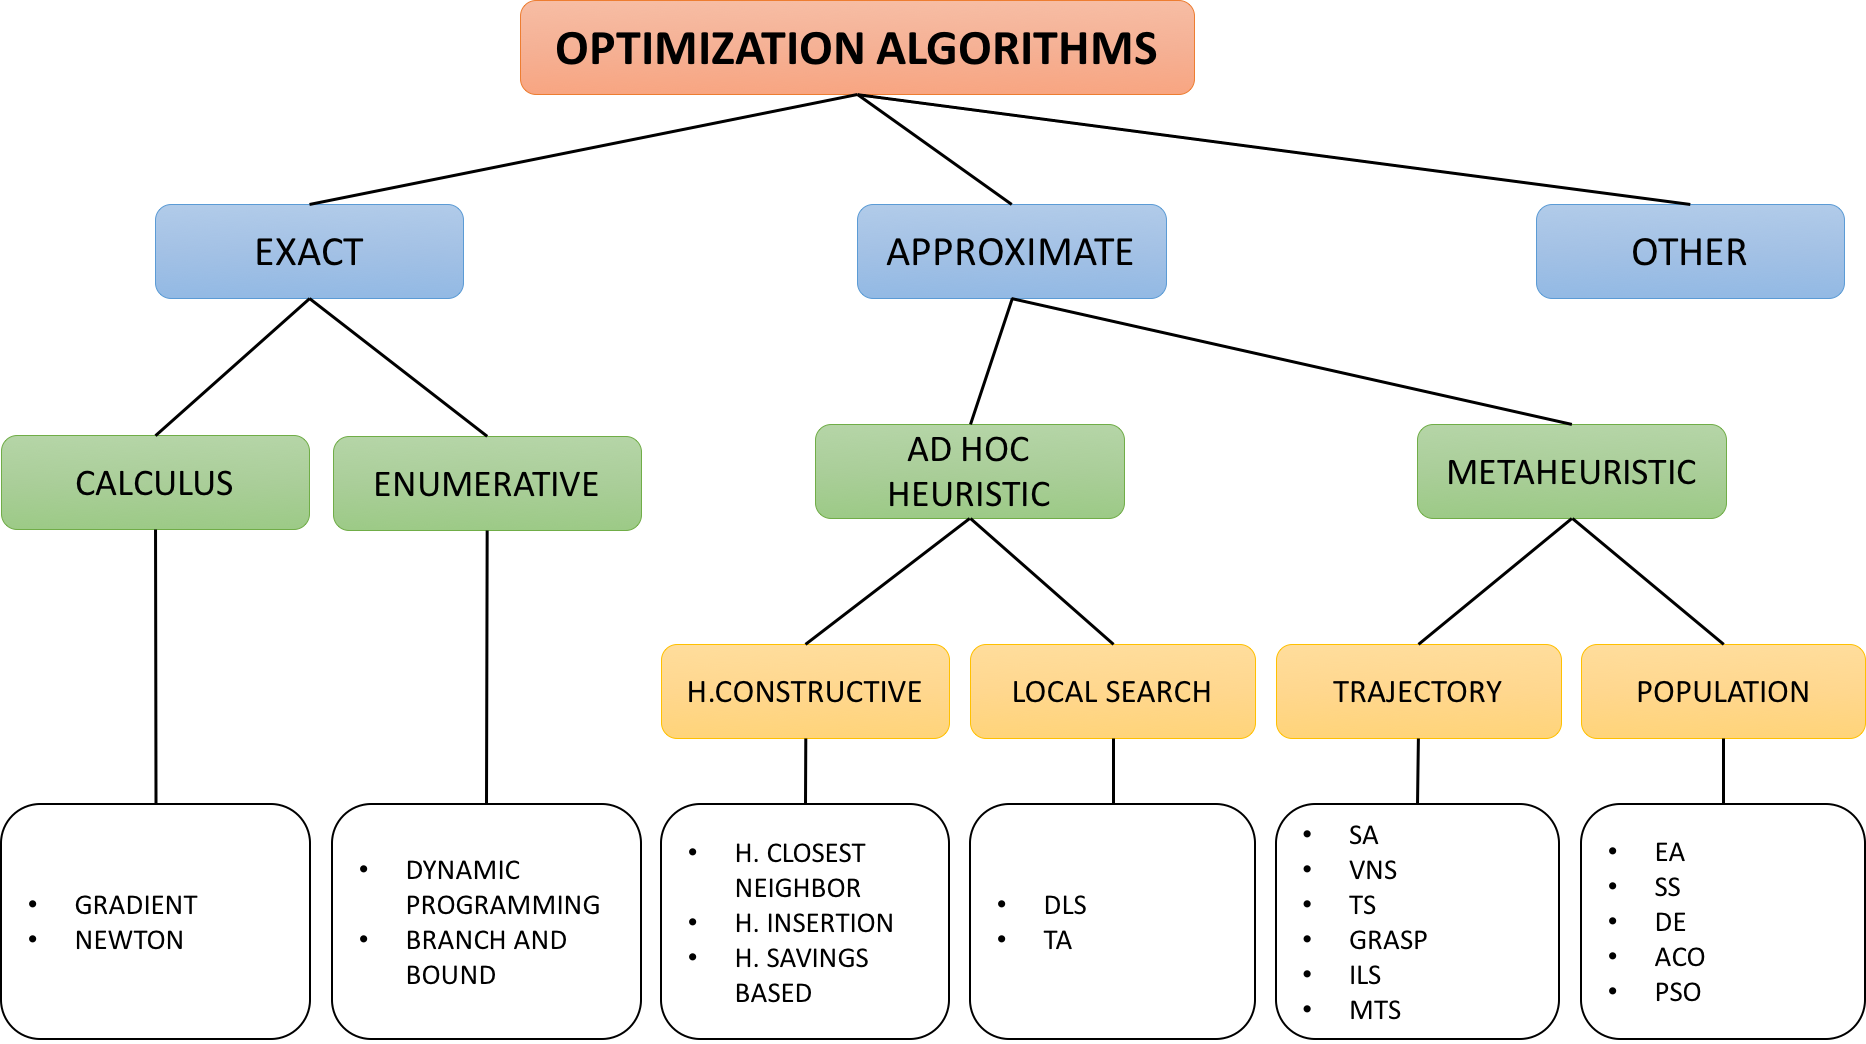
\includegraphics[width=0.80\textwidth]{img/metaheuristics/my-optimization-tech-classif.png}
	\caption{Optimization techniques classification.}\label{fig:OptTechClass} \vspace{0.5cm}
\end{figure}

Among approximate algorithms, two types can be found: \emph{ad hoc} heuristics\index{ad-hoc@\emph{ad hoc} heuristics} and metaheuristics (on which we focus on this chapter). \emph{Ad hoc} heuristics, at the same time, are divided into \emph{constructive heuristics}\index{Constructive heuristic} and \emph{local search methods}\index{Local search}.

Constructive heuristics are often the fastest methods. They build a solution from scratch by incorporating components to get a complete solution, which is the result of the algorithm. Although in many cases finding a constructive heuristic is relatively simple, the solutions offered are usually of very low quality. Finding methods of this kind that produce good solutions is very difficult, since they depend a lot on the problem, and one must have a very extensive knowledge of it for their approach. For example, when dealing with problems with many constraints, most partial solutions can only lead to non-feasible solutions.

Local search or gradient tracking methods start from a complete solution, and using the \emph{neighborhood}\index{Neighborhood} concept, explore part of the search space until finding a \emph{local optimum}\index{Local optimum}. The neighborhood of a solution $s$, that we define as $N(s)$, is the set of solutions that can be built from $s$ applying a specific modification operator (generally named \emph{movement}). A local optimum is a solution better or equal to any other solution from its neighborhood. These methods, starting from a initial solution, examine its neighborhood and they keep the best neighbor, continuing the process until finding a local optimum. In many cases, the complete exploration of the neighborhood is unfeasible and different strategies are approached, which lead to different variations of the generic scheme. According to the chosen movement operator, the neighborhood changes and the way of exploring changes as well, so the search process can be simplified or complicated.

In the 1980s a new class of approximate algorithms emerged, whose basic idea was to combine different heuristic methods at a higher level to achieve efficient and effective exploration of the search space. These techniques have been named \emph{metaheuristics}\index{Metaheuristic}. This term was introduced for the first time by Glover~\cite{glover86future}. Before the term was completely accepted by the scientific community, these techniques were called \emph{modern heuristics}\index{Modern heuristics}~\cite{reeves93modern}. This algorithm class includes techniques such as ant colonies, evolutionary algorithms, iterative local search, simulated annealing and tabu search. Metaheuristics reviews can be found in~\cite{blum03metaheuristics,glover03handbook}. From the different descriptions that can be found in the literature, several fundamental properties that characterize these types of methods can be highlighted:


\begin{itemize}
	\item Metaheuristics are general strategies or templates that guide the search process.
	
	\item The goal is an efficient exploration of the search space to find (almost) optimal solutions.
	
	\item Metaheuristics are non-accurate algorithms and are generally non-deterministic.
	
	\item They can incorporate mechanisms to avoid unpromising regions of the search space.
	
	\item The basic scheme of any metaheuristic has a predefined structure.
	
	\item Metaheuristics can make use of knowledge from the problem to be solved by using specific heuristics that are controlled by the highest level strategy.
\end{itemize}

Summarizing these points, it can be agreed that a metaheuristic is a high level strategy that uses different methods to explore the search space. In other words, a metaheuristic is a general non-deterministic template that must be filled with problem-specific data (solution representation, operators to manipulate them, etc.) and allows problems with large spaces search to be tackled. In these type of techniques is really important the correct balance (generally dynamic) that exists between \emph{diversification}\index{Diversification} and \emph{intensification}\index{Intensification}. The term diversification refers to the evaluation of solutions that are placed in distant regions of the search space (according to a previously defined distance between solutions). This term is also known as search space \emph{exploration}\index{Exploration}. The term intensification, however, refers to the evaluation of solutions in bounded and small regions from the search space centered on the neighborhood of concrete solutions (search space \emph{exploitation}\index{Explotation}). The balance between these two contrary concepts is of great importance since, on the one hand promising regions from the global search space have to be quickly identified and, on the other hand, time shouldn't be wasted in already explored regions or in those that do not contain high quality solutions.

Within metaheuristics we can distinguish two types of search strategies. First, we have the ``intelligent" extensions  of the local search methods (metaheuristics based on trajectory in Figure~\ref{fig:OptTechClass}). The goal of these strategies is to avoid in some way the local minimums and to move to other promising regions from the search space. This type of strategy is the one that is used by the tabu search\index{Tabu search}, the iterated local search\index{Iterated local search}, the variable neighborhood search\index{Variable neighborhood search} and the simulated annealing\index{Simulated annealing}. These metaheuristics work with one or several neighborhood structures imposed by the local search. Another type of strategy is the one followed by the ant colonies or the evolutionary algorithms. These ones have a learning component, in the sense that, in an implicit or explicit way, they try to learn the correlation between the problem variables in order to identify the search space regions with high quality solutions (population-based metaheuristics in the Figure~\ref{fig:OptTechClass}). These methods perform, in this sense, biased sampling of the search space.

Formally, a metaheuristic is defined as a tuple of elements that, depending on how they are defined, leads to a particular technique or another. This formal definition has been developed in~\cite{luque06resolucion} and subsequently extended in~\cite{chicano06metaheuristica}.

\index{Metaheuristic!formal definition}

\begin{definition}[Metaheuristic]
	\label{def:Metaheuristic} A metaheuristic $\mathcal{M}$ is a tuple composed by the following eight components:
	\begin{equation}
	\mathcal{M} = \langle \mathcal{T}, \Xi, \mu, \lambda, \Phi, \sigma, \mathcal{U}, \tau \rangle \enspace ,
	\end{equation}
	where:
	
	\begin{itemize}
		\item $\mathcal{T}$ is the set of elements that are handled by the metaheuristic. This set contains the search space and in most cases it coincides with it.
	
		\item $\Xi = \{ (\xi_1,D_1), (\xi_2, D_2), \ldots, (\xi_v, D_v) \}$ is a set of $v$ pairs. Each pair is composed by a state variable of the metaheuristic and by the domain of this variable.
		
		\item  $\mu$ is the number of solutions with which $\mathcal{M}$ operates in one step.
		
		\item $\lambda$ is the number of new solutions that are generated in each iteration of $\mathcal{M}$.
				
		\item $\Phi: \mathcal{T}^\mu \times \prod\limits_{i=1}^{v} D_i \times \mathcal{T}^\lambda \rightarrow [0,1]$ represents the operator that creates new solutions from the existent ones. This function must fulfill for all $x \in
		\mathcal{T}^\mu$ and for all $t \in \prod_{i=1}^{v} D_i$,
		\begin{equation}
		\label{eq:metah-phi} \sum_{y \in \mathcal{T}^\lambda} \Phi (x,t,y) = 1 \enspace .
		\end{equation}
		
		\item $\sigma: \mathcal{T}^\mu \times \mathcal{T}^\lambda \times \prod\limits_{i=1}^{v} D_i \times \mathcal{T}^{\mu}
		\rightarrow [0,1]$ is a function that allows to select those solutions that will be handled in the following iteration of  $\mathcal{M}$. This function must fulfill for all $x \in \mathcal{T}^{\mu}$, $z \in
		\mathcal{T}^{\lambda}$ y $t \in \prod_{i=1}^{v} D_i$,
		\begin{eqnarray}
		& & \sum_{y \in \mathcal{T}^\mu} \sigma (x,z,t,y) = 1 \enspace , \\
		& & \forall y \in \mathcal{T}^\mu, \sigma(x,z,t,y) = 0 \vee \\
		& & \nonumber \;\; \vee \sigma(x,z,t,y) > 0 \wedge  \\
		& & \nonumber (\forall i \in \{1,\ldots,\mu\} \bullet (\exists j \in \{1,\ldots,\mu\}, y_i=x_j) \vee (\exists j \in
		\{1,\ldots,\lambda\}, y_i=z_j)) \enspace .
		\end{eqnarray}
		
		\item $\mathcal{U}: \mathcal{T}^\mu \times \mathcal{T}^\lambda \times \prod\limits_{i=1}^{v} D_i \times
		\prod\limits_{i=1}^{v} D_i \rightarrow [0,1]$ represents the update procedure of the state variable of the metaheuristic. This function must fulfill for all $x \in \mathcal{T}^{\mu}$, $z \in \mathcal{T}^{\lambda}$ y $t
		\in \prod_{i=1}^{v} D_i$,
		\begin{equation}
		\sum_{u \in \prod_{i=1}^{v} D_i} \mathcal{U} (x,z,t,u) = 1 \enspace .
		\end{equation}
		
		\item $\tau: \mathcal{T}^\mu \times \prod\limits_{i=1}^{v} D_i \rightarrow \{false, true\}$ is a function that decides the termination of the algorithm.
		
	\end{itemize}
\end{definition}

The above definition reflects the typical stochastic behavior of metaheuristic techniques. In particular, the
$\Phi$, $\sigma$, and $\mathcal{U}$ functions must be interpreted as conditional probabilities. For example, the value of $\Phi(x,t,y)$ is interpreted as the probability that the child vector $y \in \mathcal{T}^\lambda$ is generated since at the moment the set of individuals with which the metaheuristic works is $x \in \mathcal{T}^\mu$ and its internal state is defined by the state variables $t \in \prod_{i=1}^{v} D_i$. It can be seen that the constraints imposed on the functions $\Phi$, $\sigma$ y $\mathcal{U}$ allow to consider them as functions that return these conditional probabilities.

\begin{definition}[Metaheuristic state]\index{Metaheuristic state}
	\label{def:MetaheuristicState} Let $\mathcal{M} = \langle \mathcal{T}, \Xi, \mu, \lambda, \Phi, \sigma, \mathcal{U}, \tau \rangle$ be a metaheuristic and $\Theta = \{ \theta_1, \theta_2, \ldots, \theta_\mu\}$ the set of variables that will store the solution set with which the metaheuristic works. We will use the notation $first(\Xi)$ to refer to the state variable set of the metaheuristic, $\{\xi_1,\xi_2, \ldots, \xi_v\}$. A \emph{state} $s$ of the metaheuristic is a pair of functions $s=(s_1,s_2)$ with
	\begin{eqnarray}
	& & s_1: \Theta \rightarrow \mathcal{T}, \\
	& & s_2: first(\Xi) \rightarrow \bigcup\limits_{i=1}^{v} D_i \enspace ,
	\end{eqnarray}
	where $s_2$ satisfies
	\begin{equation}
	s_2(\xi_i) \in D_i \enspace \forall \xi_i \in first(\Xi) \enspace .
	\end{equation}
	
	We will denote with $\mathcal{S}_\mathcal{M}$ the set of all states of a metaheuristic $\mathcal{M}$.
\end{definition}

Finally, once defined the state of a metaheuristic, we can define its dynamic.

\begin{definition}[Metaheuristic dynamic]\index{Metaheuristic!dynamic}
	Let $\mathcal{M} = \langle \mathcal{T}, \Xi, \mu, \lambda, \Phi, \sigma, \mathcal{U}, \tau \rangle$ be a metaheuristic and $\Theta = \{ \theta_1, \theta_2, \ldots, \theta_\mu\}$ the set of variables that will store the solution set with which the metaheuristic works. We will use the notation $\overline{\Theta}$ for the tuple $(\theta_1, \theta_2, \ldots,	\theta_\mu)$ and $\overline{\Xi}$ for the tuple $(\xi_1, \xi_2, \ldots, \xi_v)$. We will extend the state definition so that it can be applied to element tuples. Then, we define $\overline{s}=(\overline{s}_1,\overline{s}_2)$ where

	\begin{eqnarray}
	& & \overline{s}_1: \Theta^n \rightarrow \mathcal{T}^n \enspace ,\\
	& & \overline{s}_2: first(\Xi)^n \rightarrow \left(\bigcup\limits_{i=1}^{v} D_i\right)^n \enspace ,
	\end{eqnarray}
	and besides that
	%y además
	\begin{eqnarray}
	& & \overline{s}_1(\theta_{i_1},\theta_{i_2}, \ldots, \theta_{i_n}) = (s_1(\theta_{i_1}), s_1(\theta_{i_2}), \ldots, s_1(\theta_{i_n})) \enspace , \\
	& & \overline{s}_2(\xi_{j_1},\xi_{j_2}, \ldots, \xi_{j_n}) = (s_2(\xi_{j_1}), s_2(\xi_{j_2}), \ldots, s_2(\xi_{j_n}))
	\enspace ,
	\end{eqnarray}
	for $n\geq 2$. We will say that $r$ is a successor state of $s$ if $t \in \mathcal{T}^\lambda$ exists such that
	$\Phi(\overline{s}_1(\overline{\Theta}), \overline{s}_2(\overline{\Xi}), t) > 0$ and besides that
	\begin{eqnarray}
	& & \sigma(\overline{s}_1(\overline{\Theta}), t, \overline{s}_2(\overline{\Xi}), \overline{r}_1(\overline{\Theta})) > 0 \enspace y\\
	& & \mathcal{U}(\overline{s}_1(\overline{\Theta}), t, \overline{s}_2(\overline{\Xi}), \overline{r}_2(\overline{\Xi})) >
	0 \enspace .
	\end{eqnarray}
	
	We will denote with $\mathcal{F}_\mathcal{M}$ the binary relation ``being a successor of'' defined in the states set of a metaheuristic $\mathcal{M}$. That is, $\mathcal{F}_\mathcal{M} \subseteq \mathcal{S}_\mathcal{M} \times
	\mathcal{S}_\mathcal{M}$, and $\mathcal{F}_\mathcal{M}(s,r)$ if $r$ is a successor state of $s$.
\end{definition}

\begin{definition}[Metaheuristic execution]\index{Metaheuristic!execution} A metaheuristic $\mathcal{M}$ execution is a finite or infinite sequence of states, $s_0, s_1, \ldots$ in which $\mathcal{F}_\mathcal{M}(s_i,s_{i+1})$ for all $i\geq 0$ and
	besides that:
	\begin{itemize}
		\item if the sequence is infinite $\tau(s_i(\overline{\Theta}), s_i(\overline{\Xi})) = false$ is satisfied for all $i \geq 0$ and
		
		\item if the sequence is finite $\tau(s_k(\overline{\Theta}), s_k(\overline{\Xi})) = true$ if satisfied for the last state $s_k$ and, besides, $\tau(s_i(\overline{\Theta}), s_i(\overline{\Xi})) = false$ for all $i \geq 0$ such that $i < k$.
	\end{itemize}
	
\end{definition}

In the next sections we will have the opportunity to see how this general formulation can be adapted to the specific techniques (obviating those parameters not fixed by metaheuristics or that depend on other aspects such as the problem or the concrete implementation).

\section{Classification}\label{sec:MetaheuristicsClassification}

There are different ways of classifying and describing the metaheuristic techniques~\cite{blum03metaheuristics}. Depending on the selected characteristics, it is possible to obtain different taxonomies: based on nature or non based on nature, with or without memory, with one or several neighborhood structures, etc. One of the most popular classifications makes the following division: \emph{trajectory-based}\index{Metaheuristic!trayectory-based} and \emph{population-based}\index{Metaheuristic!population-based} metaheuristics. The former manipulates a single element of the search space at each step, while the latter work on a set of them (population). This taxonomy is shown graphically in the Figure~\ref{fig:MetaheuristicsClassification}, which also includes the most representative techniques. These metaheuristics are described in the two following sections.

\begin{figure}[H] %tb
	\centering
	\vspace{0.5cm} \centering 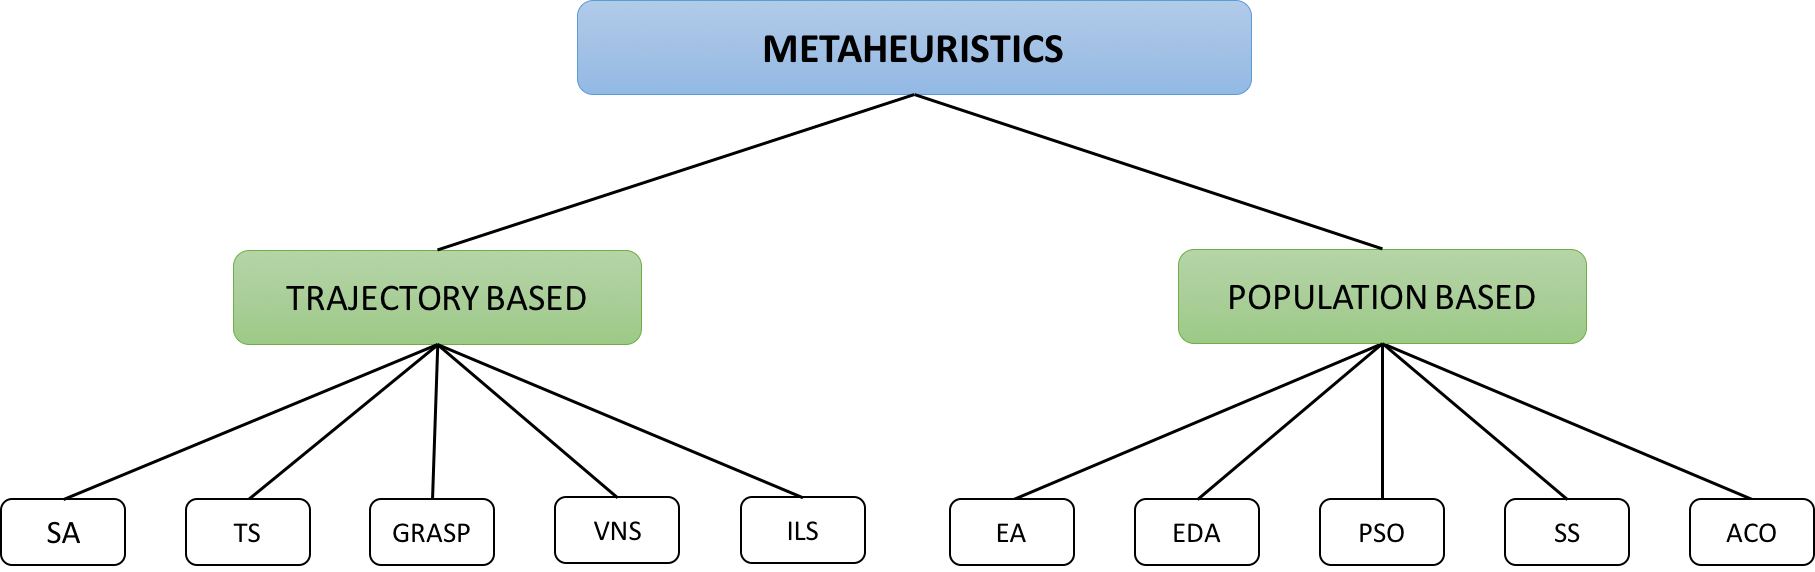
\includegraphics[width=0.80\textwidth]{img/metaheuristics/my-metaheuristics-classif.png} 
	%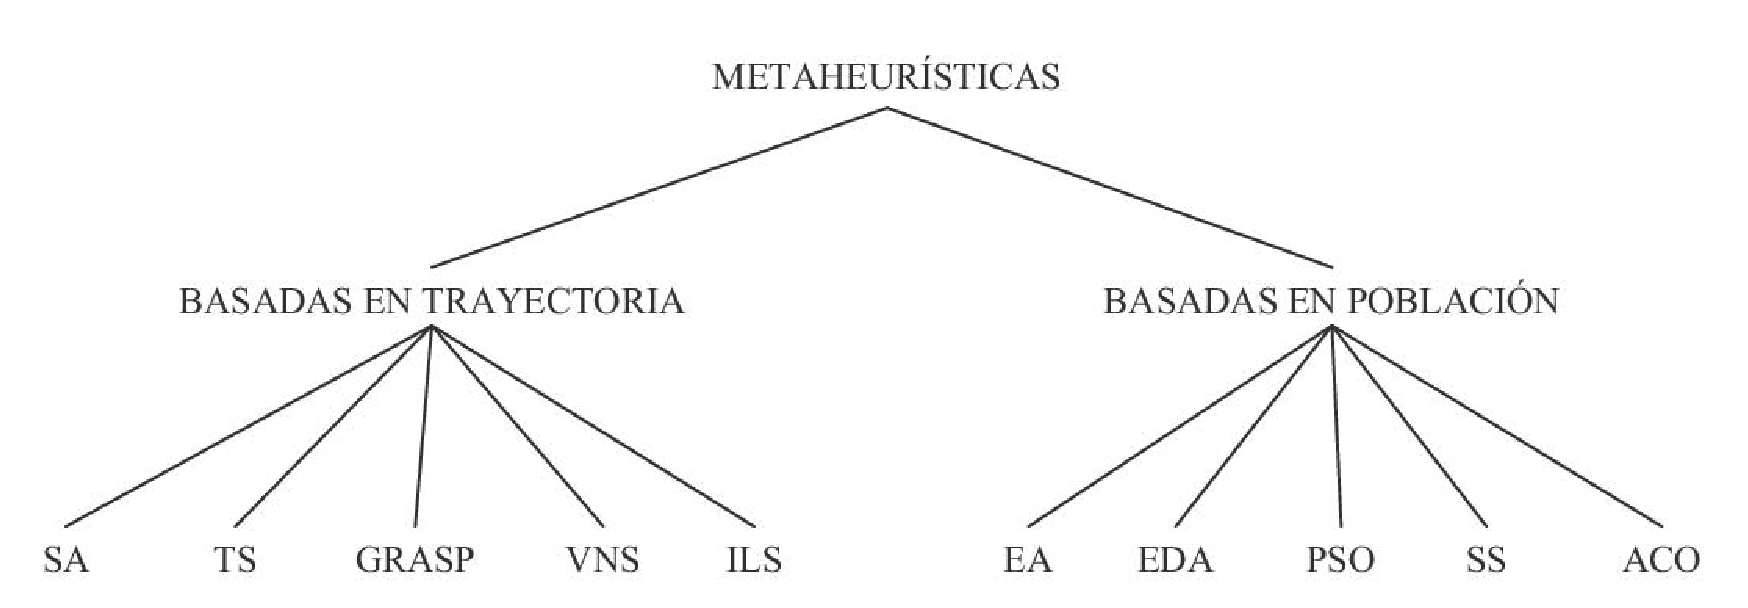
\psfig{file=./img/metaheuristics/clasif-metah,width=14cm} 
	\caption{Metaheuristics classification.}\label{fig:MetaheuristicsClassification}
\end{figure}


\subsection{Trajectory-based metaheuristics}
\label{sec:TrajectoryBasedMetaheuristics}
\index{Metaheuristic!trayectory-based}

In this section, we will briefly review some metaheuristics based on trajectory. The main characteristic of these methods is that they start from a solution and, through the neighborhood exploration, they update the current solution, forming a trajectory. According to the notation of Definition~\ref {def:Metaheuristic}, this is formalized with $\mu = 1$. Most of these algorithms arise as extensions of simple local search methods to which some mechanism is added to escape local minimums. This implies the need for a more elaborated stopping condition than finding a local minimum. Usually the search is terminated when a predefined maximum number of iterations is reached, a solution with an acceptable quality is found, or a stagnation of the process is detected.

\subsubsection{Simulated Annealing (SA)}

\emph{Simulated annealing}\index{Simulated annealing} (SA) is one of the oldest techniques between metaheuristics and is possibly the first algorithm with an explicit strategy to escape from the local minimum. The algorithm origins are found in an statistic mechanism named \emph{metropolis}~\cite{metropolis53equation}. The SA idea is to simulate the cooling process of metal and crystal. SA was initially introduced in~\cite{kirkpatrick83optimization}. In order to avoid being trapped in a local minimum, the algorithm allows to choose, with  a determined probability, a solution whose value of \emph{fitness} is worse than that of the current solution. In each iteration, a solution $s'$ of the neighborhood $N(s)$ is chosen from the current solution $s$. If $s'$ is better than $s$ (that is, it has a better value in the \emph{fitness} function), $s$ is substituted for $s'$ as the current solution. If the solution $s'$ is worse, then it is accepted with a certain probability that depends on the current temperature $T$ and the difference of \emph{fitness} between both solutions,
$F(s') - f(s)$ (case of minimization). 

\subsubsection{Tabu search (TS)}

\emph{Tabu search}\index{Tabu search} (TS) is one of the metaheuristics that have been applied more successfully when solving combinatorial optimization problems. These method fundamentals were introduced in~\cite{glover86future}, and are based on the ideas formulated in~\cite{glover77heuristics}. A good summary of this technique and its components can be found in~\cite{glover77heuristics}.

The basic idea of the tabu search is the explicit use of a search record (a short-term memory), both to escape local minima and to implement its exploration strategy, and to avoid searching several times in the same region. This short-term memory is implemented as a tabu list, where the more recently visited solutions are kept to exclude them from the next movements. In each iteration the best solution is chosen among the allowed ones and is added to the tabu list.

From the point of view of implementation, maintaining a list of complete solutions is often impractical due to its inefficiency. Therefore, generally, movements that had led the algorithm to generate that solution or the main components that define the solution are usually stored. In any case, the elements of this list allow filtering the neighborhood, generating a reduced set of eligible solutions called $N_a(s)$. The store of movements instead of complete solutions is much more efficient, but introduces a loss of information. To avoid this problem, an aspiration criterion is defined which allows to include a solution in $N_a(s)$ even if it is prohibited due to the tabu list. The most widely used aspiration criterion is to allow solutions whose \emph{fitness} is better than the best solution found so far.

\subsubsection{GRASP}

The \emph{Greedy Randomized Adaptive Search Procedure}\index{GRASP} (GRASP) \cite{feo95greedy} is a simple metaheuristic that combines constructive heuristics with local search. GRASP is an iterative procedure, composed of two phases: first the construction of a solution and then an improvement process. The improved solution is the result of the search process. The solution-building mechanism is a random constructive heuristic. It adds step by step different components $c$ to the partial solution $s^p$, which is initially empty. The components added in each step are randomly selected from a restricted list of candidates ($RCL$). This list is a subset of $N(s^p)$, the set of allowed components for the partial solution $s^p$. To generate this list, the components of the solution in $N(s^p)$ are ordered according to some function dependent on the problem ($\eta$).

The $RCL$ list is composed by the $\alpha$ best components of that set. In the extreme case of $\alpha = 1$, we always add the best found component deterministically, so that the construction method is equivalent to a voracious algorithm. At the other end, with $\alpha = |N(s^p)|$, the component to be added is chosen in a totally random way from all available ones. Therefore, $\alpha$ is a key parameter that influences how the search space is to be sampled. The second phase of the algorithm consists in applying a local search method to improve the generated solution. This enhancement mechanism may be a simple enhancement technique or other more complex algorithms such as SA or TS.

\subsubsection{Variable Neighborhood Search (VNS)}

The \emph{Variable Neighborhood	Search}\index{Variable Neighborhood Search} (VNS) is a metaheuristic proposed in~\cite{mladenovic97variable} which applies explicitly one strategy to change between different neighborhoods during the search. This algorithm is very general and with many degrees of freedom when designing particular variations and instantiations.

The first step is to define a set of neighborhoods. This choice can be made in many ways: from being randomly chosen to using complex equations deduced from the problem. Each iteration consists of three phases: the candidate's choice, a phase of improvement and, finally, the movement. In the first phase, a neighbor $s'$ of $s$ is chosen randomly using the $k$-th neighborhood. This solution $s'$ is used as the starting point of the local search of the second phase. When the improvement process ends, the new $s''$ solution is compared to the original $s$. If it is better, $s''$ becomes the current solution and the neighborhood counter is initialized ($k \leftarrow 1$). If it is not better, the process is repeated but using the following neighborhood ($ k \leftarrow k+1 $). The local search is the intensification step of the method and the neighborhood change can be considered as the diversification step.

\subsubsection{Iterated Local Search (ILS)}

The \emph{Iterated Local Search}\index{Iterated local search} (ILS)
\cite{loureco02iterated,stutzle99ILS} is a metaheuristic based in a simple but very effective concept. In each iteration, the current solution is disturbed, and then, a local search method is applied to this solution to improve it. The local minimum obtained by the improvement method can be accepted as the current new solution if it passes an acceptance test. The importance of the disturbance process is obvious: if it is too small, the algorithm may not be able to escape the local minimum; however, if it is too large, the disturbance can make the algorithm behaves as a local search method with a random restart. Therefore, the perturbation method must generate a new solution that serves as a start to the local search, but that should not be very far from the current one so that it is not considered to be a random solution. The acceptance criterion acts as a counterbalance, since it filters the acceptance of new solutions depending on the search history and the characteristics of the new local minimum.

\subsection{Population-based metaheuristics}\label{sec:PopulationBasedMetaheuristics}

\index{Metaheuristics!population-based}
The population-based methods are characterized by work with a solution set, usually called population, in each iteration (that is, generally $\mu > 1$ and/or $\lambda > 1$), as opposed to methods based in trajectory, that only manipulate a solution of the search space by iteration.

\subsubsection{Evolutionary Algorithms (EA)}\label{sec:EAs}

\emph{Evolutionary algorithms}\index{Evolutionary algorithm} (EAs) are inspired by the natural evolution theory. This family of techniques follows an iterative and stochastic process that operates on a solution population, named in this context \emph{individuals}. Initially, the population is typically generated randomly (perhaps with the help of a construction heuristic).

The general scheme of an evolutionary algorithm comprises three main phases: selection, reproduction and replacement. The entire process is repeated until some termination criterion is met (usually after a given number of iterations). In the selection phase, the most suitable individuals of the present population are generally chosen to be subsequently recombined in the reproduction phase. Individuals resulting from recombination are altered by a mutation operator. Finally, from the current population and/or the best individuals generated (according to their value of \emph{fitness}) the new population is formed, giving way to the next generation of the algorithm.

\subsubsection{Estimation of Distribution Algorithms (EDA)}

\emph{Estimation of Distribution Algorithms}\index{Estimation of distribution algorithm} (EDAs) \cite{muhlenbein98equation} show a similar behavior to the evolutionary algorithms presented in the previous section. In fact, many authors consider the EDAs as another type of EA. The EDAs operate on a population of tentative solutions such as evolutionary algorithms but, unlike the latter, which use recombination and mutation operators to improve the solutions, EDAs infer the probability distribution of the selected set and, using it, they generate new solutions that will be part of the population.

Probabilistic graphical models are tools commonly used in the context of the EDAs to efficiently represent the probability distribution. Some authors \cite{larra99optimization, pelikan99boa, soto99introducing} have proposed the Bayesian networks to represent the probability distribution in discrete domains, whereas the gaussian networks are usually used in the continuous domains \cite{whittaker90graphical}.

\subsubsection{Scatter Search (SS)}

\emph{Scatter Search}\index{Scatter search} (SS)~\cite{glover98template} is a metaheuristic whose principals were introduced in \cite{glover77heuristics} and which nowadays is receiving a great deal of attention from the scientific community \cite{laguna03scatter}. The algorithm is based on maintaining a relatively small set of tentative solutions (called reference set or \emph{RefSet}) that is characterized by containing quality and diverse solutions (distant in the search space). For the complete definition of SS, five components must be defined: creation of the initial population, generation of the reference set, generation of subsets of solutions, method of combining solutions and improvement method.

\subsubsection{Ant Colony Optimization (ACO)}

The \emph{Ant Colony Optimization}\index{Ant colony optimization} (ACO) \cite{dorigo92optimization,dorigo03ant} algorithms are inspired by the behavior of real ants when looking for food. This behavior is described as follows: initially, ants explore the area near their nest randomly. As soon as an ant finds food, it takes it to the nest. While performing this path, the ant is depositing a chemical called pheromone. This substance will help the rest of the ants find the food. Indirect communication between ants through the pheromone trail enables them to find the shortest path between the nest and the food. This behavior is the one that tries to simulate this method to solve optimization problems. The technique is based on two main steps: construction of a solution based on the behavior of an ant and update of the artificial pheromone traces. The algorithm does not set any \emph{a priori} planning or synchronization between phases, and can even be performed simultaneously.

\subsubsection{Particle Swarm Optimization (PSO)}

\emph{Particle Swarm Optimization}\index{Particle swarm optimization} (PSO)~\cite{kennedy99small} algorithms are inspired by the social behavior of the flight of flocks of birds or the movement of fish banks. The PSO algorithm maintains a set of solutions, also called \emph{particles}, that are randomly initialized in the search space. Each particle has a position and velocity that changes as the search progresses. The particle movement is influenced by its velocity and by the positions where the particle itself and others in its neighborhood have found good solutions. In the context of PSO, the \emph{neighborhood of a particle} \index {neighborhood of a particle} is defined as a set of particles in the cluster. It should not be confused with the neighborhood concept of a solution previously used in this chapter. The neighborhood of a particle can be \emph{global}\index{Global neighborhood}, in which all cluster particles are considered neighbors, or \emph{local}\index{Local neighborhood}, where only the nearest particles are considered to be neighbors.


\section{Multi-objective optimization metaheuristics}
\label{sec:MOOptimizationMetaheuristics}

Most real-world optimization problems are multiobjective in nature, which means that you have to minimize or maximize several functions at the same time as they are normally in conflict with each other (multi-objective problems or MOPs, \emph{Multi-objective Optimization Problems})\index{Multi-objective optimization!MOP}. Due to the lack of adequate methodological solutions, multi-objective problems have been solved in the past as single-objective problems. However, there are fundamental differences in the operating principles of algorithms for single- and multi-objective optimization. Thus\index{Multi-objective optimization}, the techniques used to solve MOPs are not usually restricted to finding a single solution, but a set of compromise solutions between the multiple conflicting objectives, since there is usually no solution that simultaneously optimizes all objectives. Two stages can therefore be distinguished when addressing this type of problem: on the one hand, the optimization of several objective functions involved and, on the other hand, the decision-making process on which compromise solution is most appropriate \cite{coello07evolutionary}. Given how they handle these two stages, techniques for solving MOPs can be classified in \cite{cohon75review}:

\begin{itemize}
	\item \emph{A priori}: when decisions are taken before searching solutions.
	\item \emph{Progresives}: when the search for solutions and decision-making are integrated.
	\item \emph{A posteriori}: when searching is done before making decisions.
\end{itemize}

Each of them has certain advantages and disadvantages that make them more suitable for certain concrete scenarios ~\cite{coello07evolutionary, deb01multiobjective}. However, in the first two classes, the search is heavily influenced by an expert (\emph{decision maker})\index{Multi-objective optimization!Decision maker} that determines the importance of one objective over another and that can arbitrarily limit the search space, preventing an optimal resolution of the problem. In the \emph{a posteriori} techniques, on the contrary, an exploration is made as wide as possible to generate as many compromise solutions as possible. It is, then, when the decision-making process by the expert takes place. Precisely, because of this approach, these \emph{a posteriori} techniques are being used in the field of metaheuristics and, particularly, in the field of evolutionary computing \cite{coello07evolutionary, deb01multiobjective}. More specifically, the most advanced algorithms apply \emph{a posteriori} techniques based on the concept of \emph{Pareto Optimality} \cite{pareto96cours} and this is the approach followed in this thesis. Thus, we have structured this section into three sections. The first one presents formally the basic concepts related to this Pareto optimality. The following section presents the goals that should be pursued by any algorithm that uses these techniques when approaching a MOP. Finally, the third section discusses some aspects of design that must be adopted in the algorithms that solve problems following the previous approach.

\subsection{Basic concepts}
\label{ssec:MOBasicConcepts}

In this section, we present some basic concepts of multi-objective optimization to familiarize the reader with this field. We will begin by giving some notions of what we mean by multi-objective optimization problem or MOP. Informally, an MOP can be defined as the problem of finding a vector of decision variables that satisfies a set of constraints and that optimizes a set of objective functions. These functions form a mathematical description of performance criteria that are usually in conflict with each other. Therefore, the term ``optimization'' refers to the search for a solution such that it contains acceptable values for all objective functions \cite{osyczka85multicriteria}.

Mathematically, the MOP formulation extends the classical definition of single-objective optimization (Definition~\ref{def:OptimizationProblem}) to consider the existence of several objective functions. Therefore, there is not a single solution to the problem, but a solution set. This set of solutions is found by using the Pareto Optimality Theory \cite{ehrgott05multicriteria}. Formally \cite{veldhuizen99phd}:

\begin{definition}[MOP]
	\label{def:MOP} Finding a vector $\vec{x}^*= \left[x_1^*, x_2^*, \ldots,x_n^* \right]$ that satisfies the $m$
	inequality constraints $g_i\left(\vec{x}\right) \geq 0, i= 1,2,\ldots,m$, the $p$ equality constraints
	$h_i\left(\vec{x}\right) = 0, i= 1,2,\ldots,p$, and that minimizes the vector function \sloppy $\vec{f}\left(\vec{x}\right) = \left[f_1(\vec{x}),f_2(\vec{x}), \ldots , f_k(\vec{x}) \right]^T$, where $\vec{x} = \left[x_1,x_2,\ldots,x_n \right]^T$ is the decision variables vector.
\end{definition}

The set of all values satisfying the constraints defines the \emph{feasible solutions region} $\Omega$ and any point in $\vec{x} \in \Omega$ is a \emph{feasible solution}.

Having several objective functions, the notion of ``optimum'' changes, since the goal for any MOP is to find good compromises (\emph{trade-offs}) between these functions. The most used ``optimum'' notion is the one proposed by Francis Ysidro Edgeworth~\cite{edgeworth81mathematical}, later generalized by Vilfredo Pareto~\cite{pareto96cours}. Although some authors call it the Edgeworth-Pareto optimum, the Pareto optimum term is commonly accepted. Its formal definition is given as follows:\index{Pareto optimality}

\begin{definition}[Pareto optimality] \label{def:ParetoOptimum}A point $\vec{x}^* \in \Omega$ is a Pareto optimum if for each $\vec{x} \in \Omega$ and $I = \left\{1,2,\ldots,k \right\}$, or $\forall_{i \in I} \left( f_i \left(
	\vec{x} \right) = f_i(\vec{x}^*) \right)$ or there is at least one $i \in I$ $|$ $f_i\left(\vec{x}\right) >
	f_i\left(\vec{x}^*\right)$.
\end{definition}

This definition says that  $\vec{x}^*$ is a Pareto optimum if there is not any feasible vector  $\vec{x}$ that improves any criterion without simultaneously causing a worsening in at least one other criterion (assuming minimization). The Pareto optimality concept is integral to both the theory and the resolution of MOPs. There are a few additional definitions that are also basic in multi-objective optimization \cite{veldhuizen99phd}:

\begin{definition}[Pareto dominance] \label{def:ParetoDominance} A vector $\vec{u} = \left(u_1, \ldots, u_k \right)$ is said to dominate another vector $\vec{v}\!\! =\!\! \left(v_1, \ldots, v_k \right)$ (represented by $\vec{u} \prec \vec{v}$) if and only if $\vec{u}$ is partially less than \sloppy $\vec{v}$, that is, $\forall i \in \left\{1, \ldots, k \right\}, \; u_i \leq v_i \;\wedge \; \exists \; i \in \left\{1, \ldots, k \right\}: \; u_i < v_i.$
\end{definition} \index{Pareto dominance}

\begin{figure}[H] %t
	\centering 
	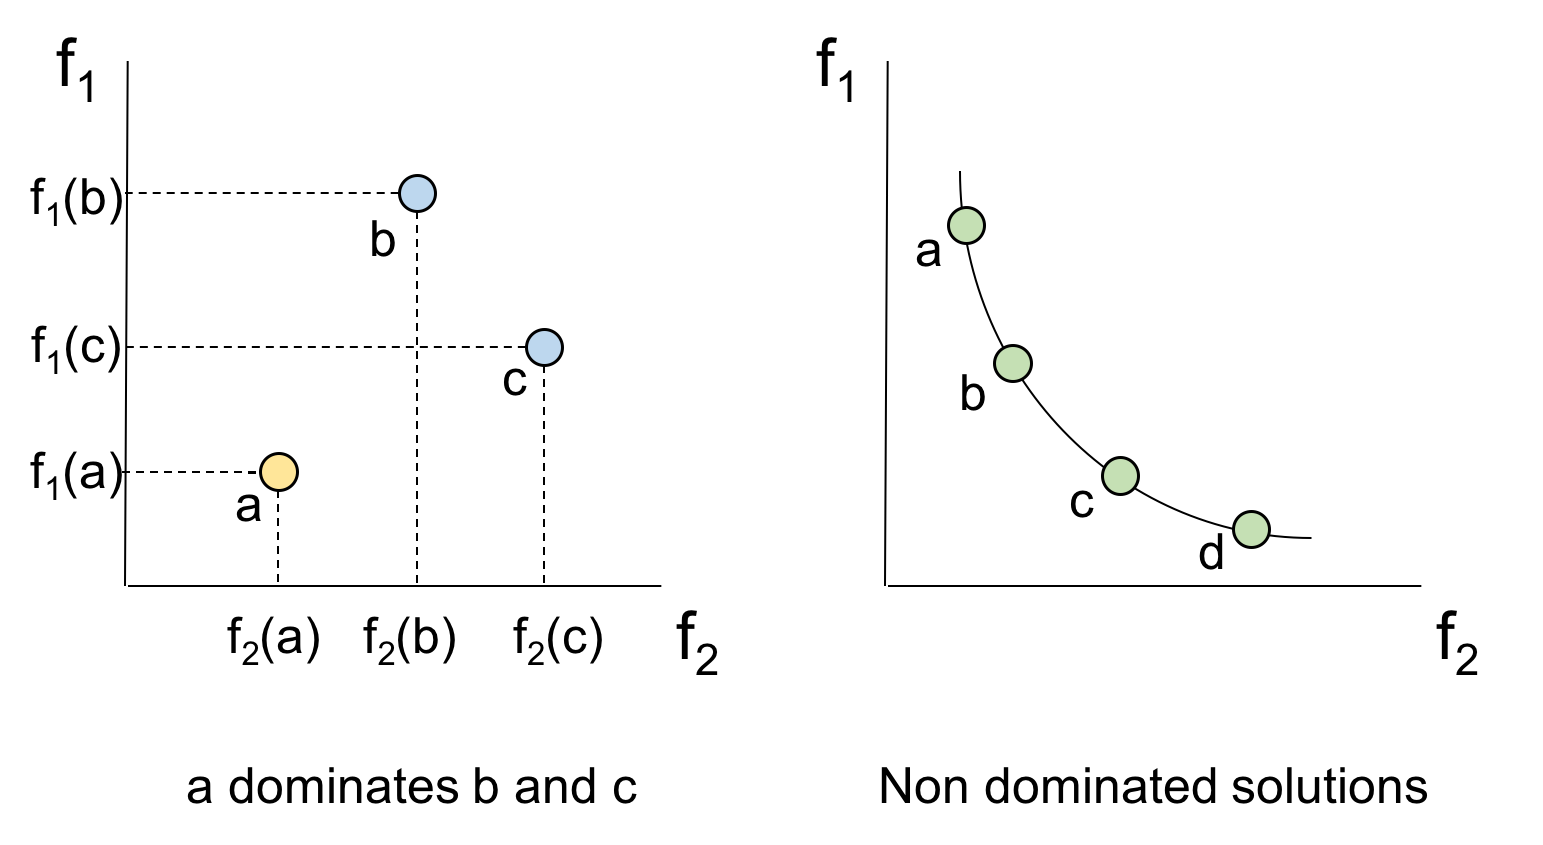
\includegraphics[width=0.80\textwidth]{img/metaheuristics/my-dominance.png}
	%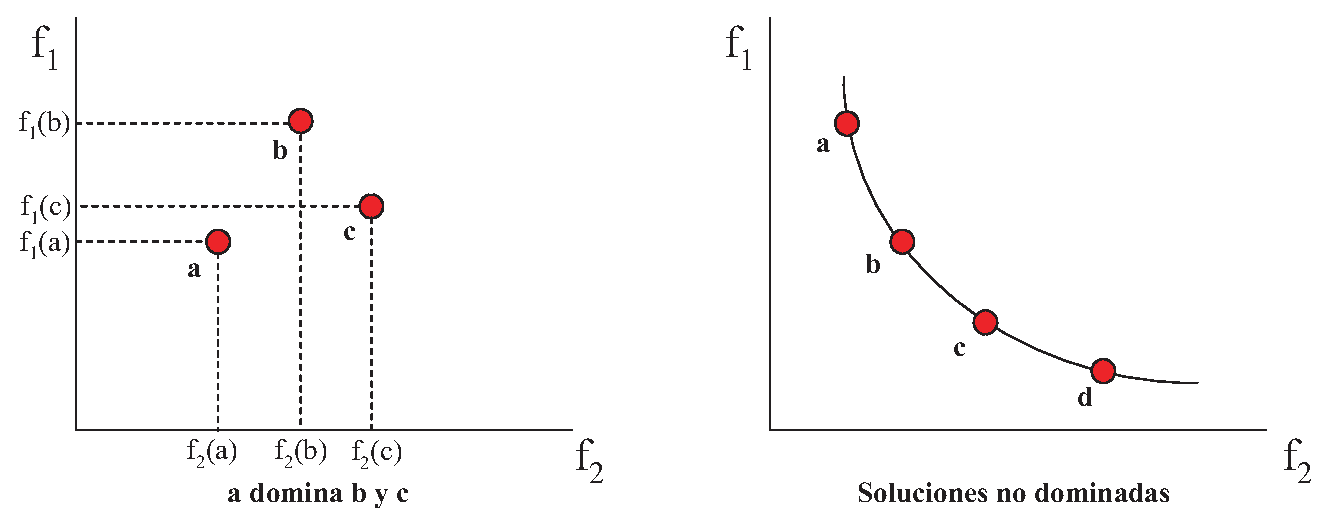
\epsfig{file=./img/metaheuristics/dominancia, width=14cm}
	\caption{Pareto dominance example.} \label{fig:dominance}
\end{figure}


We are going to illustrate this concept graphically. Figure~\ref {fig:dominance} includes two sets of solutions for a multi-objective problem with two functions $f_1$ and $f_2$, which have to be minimized. Both objectives being equally important, it is not trivial to distinguish which solution is better than another. We can use the above definition for this. Thus, if we look at the left side of the figure, we can say that $a$ is better than $b$ since $f_1(a) < f_1(b)$ and $f_2(a) < f_2(b)$. That is, it is better in both objectives and, therefore, it is said that $a$ dominates $b$ ($a \prec b$). The same happens if we compare $a$ and $c$, in both objectives $f_1 (a) < f_1(c)$ and $f_2(a) < f_2(c)$, so $a \prec c$. Let us now compare the solutions $b$ and $c$ between them. It can be seen that $c$ is better than $b$ in $f_1$ ($f_1(c) < f_1(b)$), but $b$ is better than $c$ for $f_2$ ($f_2(b) < f_2 (c)$). According to the Definition \ref{def:ParetoDominance}, we can not say that $b$ dominates $c$ nor that $c$ dominates $b$. That is, we cannot conclude that one solution is better than the other, in which case both solutions are said to be non-dominated. In the right-hand part of the Figure~\ref{fig:dominance}, 4 solutions of this type are shown, where none is better than the others.

Solving a MOP consists, therefore, of finding the set of solutions that dominate any other solutions from the solution space, which means that they are the best solutions for the problem and, therefore, make up its optimal solution. Formally:

\begin{definition}[Pareto optimal set] \label{def:ParetoOptimalSet} For a given MOP $\vec{f}(\vec{x})$,
	the Pareto optimal set is defined as $\mathcal{P^*} = \{\vec{x} \in \Omega | \neg\exists\vec{x'} \in \Omega,
	\vec{f}(\vec{x'}) \preccurlyeq \vec{f}(\vec{x})\}$.\index{Pareto optimal set}
\end{definition}

It should not be forgotten that Pareto-optimal solutions (which  are in $\mathcal{P^*}$), are in the variables space (genotype). Their vector components are in the objective space (phenotype) and they can not be improved simultaneously. These solutions are also often called \emph{not lower}, \emph{admissible} or \emph{efficient}. The Pareto front is then defined as:

\begin{definition}[Pareto front]
	\label{def:ParetoFront} For a given MOP $\vec{f}(\vec{x})$ and its Pareto optimal set $\mathcal{P^*}$, the Pareto front is defined as $\mathcal{PF^*} = \{\vec{f}(\vec{x}), \vec{x} \in \mathcal{P^*} \}$. \index{Pareto front}
\end{definition}

\begin{figure}[H] %t
	\centering
	%\begin{small}
	\begin{tabular}{|c | c|}
		\hline \scriptsize $\begin{array}{l l l l}
		$Min $ F &=& (f_1(\vec{x}), f_2(\vec{x})) \\
		f_1(\vec{x}) &=& 4x_1^2 + 4x_2^2  \\
		f_2(\vec{x}) &=& (x_1 - 5)^2 + (x_2 - 5)^2  \\
		\\
		\mbox{Subject to:} \\
		\\
		\multicolumn{1}{r}{g1(\vec{x})} &  =   & \multicolumn{1}{c}{(x_1 - 5)^2 + x_2^2 - 25}         & \multicolumn{1}{r}{\leq 0}  \\
		\multicolumn{1}{r}{g2(\vec{x})} &  =   & \multicolumn{1}{c}{-(x_1 - 8)^2 - (x_2+ 3)^2 +  7.7} & \multicolumn{1}{r}{\leq 0}  \\
		\multicolumn{1}{r}{0}           & \leq & \multicolumn{1}{c}{x_1}                              & \leq 5 \\
		\multicolumn{1}{r}{0}           & \leq & \multicolumn{1}{c}{x_2}                              & \leq 3  \\
		\end{array}$
		
		&
		
		\begin{minipage}{5cm}
			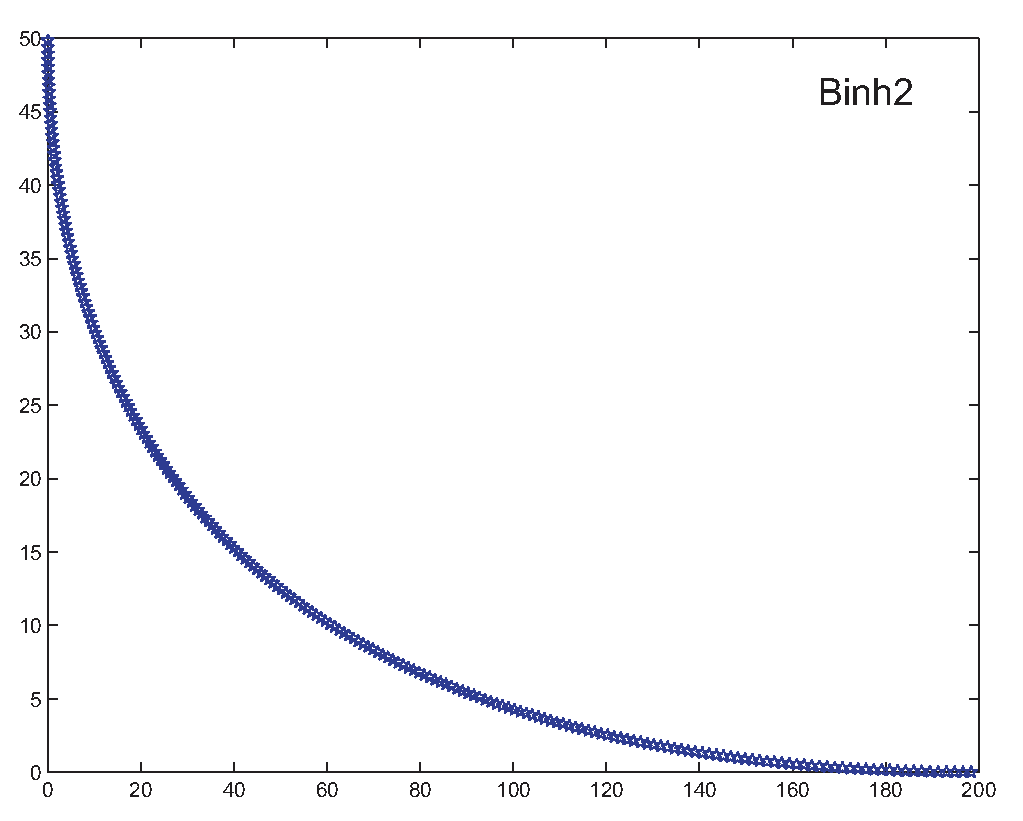
\epsfig{file=./img/metaheuristics/Binh2-1000, width=5cm}
		\end{minipage} \\ \hline
	\end{tabular}
	\caption{Formulation and Pareto front for the Bihn2 problem.} \label{fig:ExampleBihn2}
\end{figure}

%\vspace{0.5cm}

\begin{figure}[H] %!t
	\centering
	%\begin{small}
	\begin{tabular}{|c | c|}
		\hline \scriptsize $\begin{array}{l l l}
		f_1(x) &=& (1 + g(x_M)) \cos (x^\alpha_1 \frac{\pi}{2} ) \cos (x^\alpha_{2} \frac{\pi}{2}) \\
		f_2(x) &=& (1 + g(x_M)) \cos (x^\alpha_1 \frac{\pi}{2} ) \sin (x^\alpha_{2} \frac{\pi}{2}) \\
		f_3(x) &=& (1 + g(x_M))\sin(x^\alpha_1 \frac{\pi}{2}) \\
		& & 0 \leq x_i \leq 1, \;\; i = 1,2, \ldots, n \\
		\\
		
		g(x_M)&  = & \sum_{x_i \in x_M}{(x_i - 0.5)^2}  \\
		& & \\
		n      & = & 12 \\
		x_M    & = & x_3, ..., x_{12} \\
		\alpha & = & 100 \\
		%  & & \\
		\end{array}$
		
		&
		
		\begin{minipage}{6cm}
			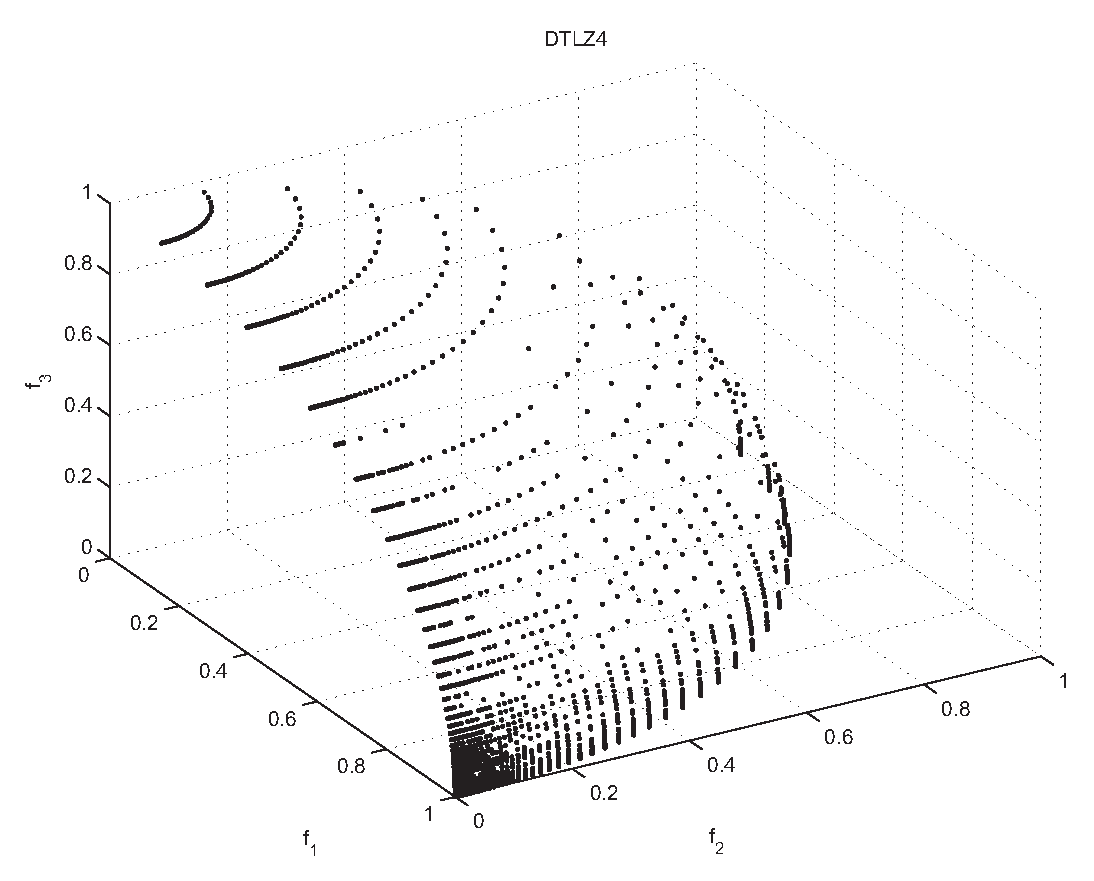
\epsfig{file=./img/metaheuristics/dtlz4, width=5.5cm}
		\end{minipage} \\ \hline
	\end{tabular}
	\caption{Formulation and Pareto front for the DTLZ4 problem.} \label{fig:ExampleDTLZ4}
\end{figure}

That is, the Pareto front is composed of the values in the objective space of the Pareto optimal set. In general, it is not easy to find an analytical expression of the line or surface that contains these points. In fact, in most cases it is impossible. As an example, Figures~\ref{fig:ExampleBihn2} and~\ref{fig:ExampleDTLZ4} show the formulation and its corresponding Pareto front of problems Binh2 and DTLZ4~\cite{coello07evolutionary}. In the first case, it is a bi-objective problem, $f_1$ and $f_2$, with two decision variables $x_1$ and $x_2$, which has two constraints defined as $g1$ and $g2$. The DTLZ4 problem, however, has three objectives and no constraint (the $g()$ function here is only a notation used for its formulation).

\subsection{Objectives in MOPs resolution} \label{ssec:Objectives}

When addressing the resolution of a multi-objective optimization problem, the main goal of any optimization algorithm that uses the concepts and techniques described in the previous section is to find its Pareto front (or, what is the same, its Pareto optimal set). However, the presence of multiple Pareto-optimal solutions makes it difficult to choose one solution over another without additional information on the problem, since all these solutions are equally important. Given a MOP, therefore, we are ideally looking for a number of non-dominated solutions that pursues two goals:

\begin{enumerate}
	\item To find a set of solutions as close as possible to the optimal Pareto front.
	\item To find a set of solutions as uniformly diverse as possible.
\end{enumerate}

While the first goal, converging towards the optimal solution, is mandatory in all tasks of single- or multi-objective optimization, the second one is completely specific for multi-objective optimization. Besides converging towards the optimum front, the solutions must be uniformly distributed along the whole front. Only with a diverse set of solutions can we ensure, on the one hand, a good set of compromise solutions between the different objectives for the subsequent decision-making by the expert and, on the other hand, that a good exploration of the search space has been made. Figure~\ref{fig:conv.fail.div.ok} shows two examples of fronts each failing in one of the previous goals. In part (a) we can see an approximation to the front in which the non-dominated solutions are perfectly distributed. However, it is a MOP designed in a way that contains multiple misleading fronts and, in fact, the solutions obtained are not Pareto-optimal, although their diversity is excellent. On the contrary, in part (b) of the same figure, we have a solution set that have converged towards the Pareto optimal front, but nevertheless some regions are left uncovered. Although neither case is desirable, the first situation is clearly worse: none of the obtained solutions is Pareto-optimal.

\begin{figure}[H] %!t
	\centering
	\begin{tabular}{cc}
		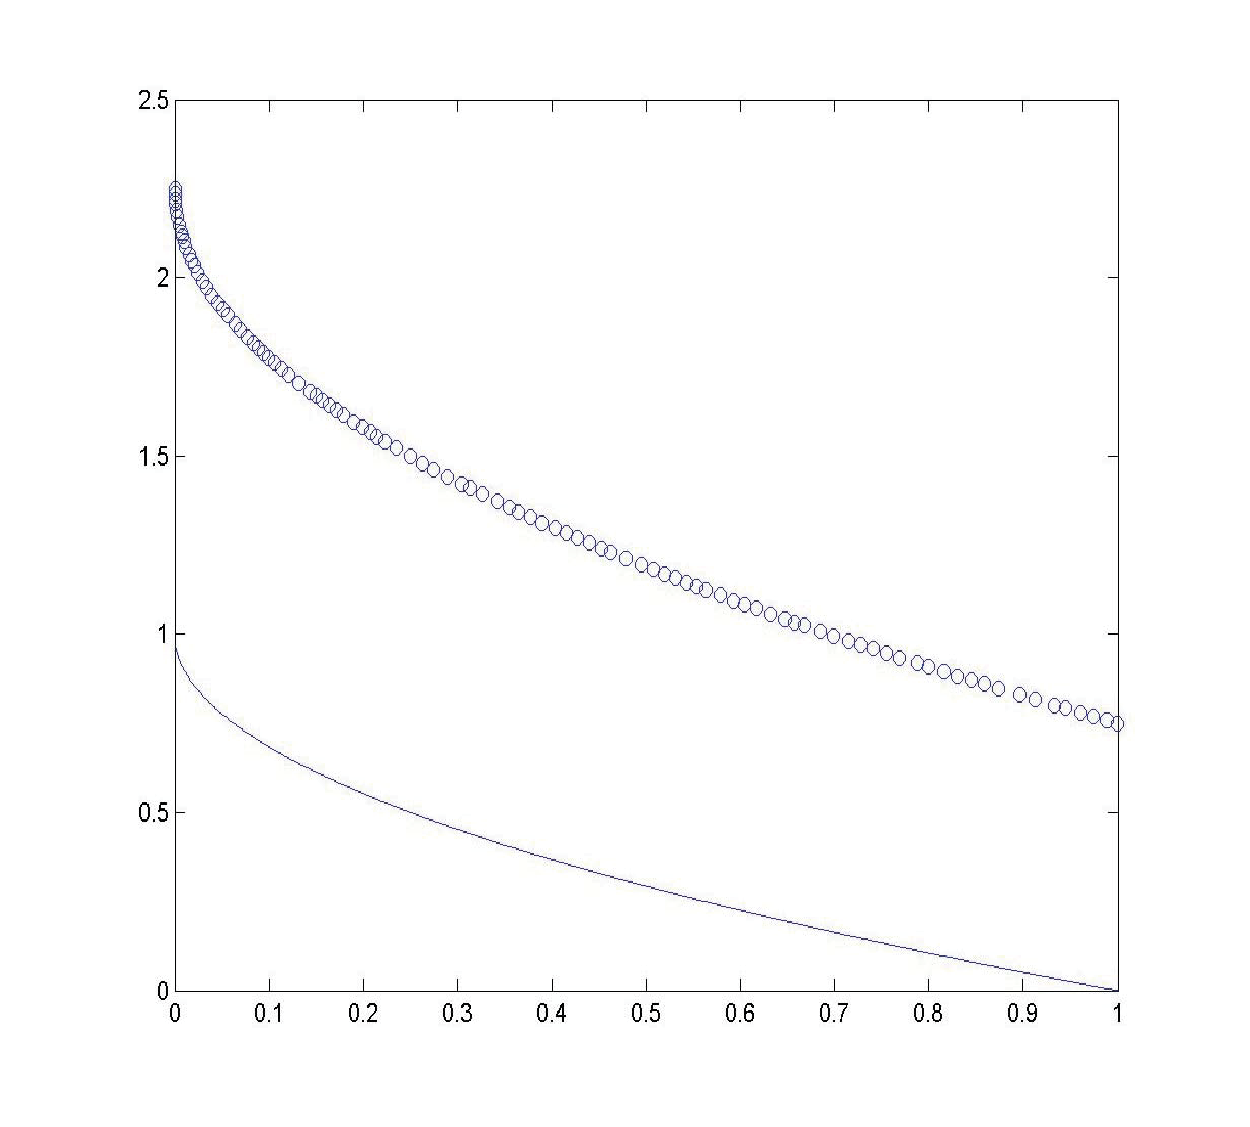
\epsfig{file=./img/metaheuristics/conv-fail-div-ok, width=6.5cm} &
		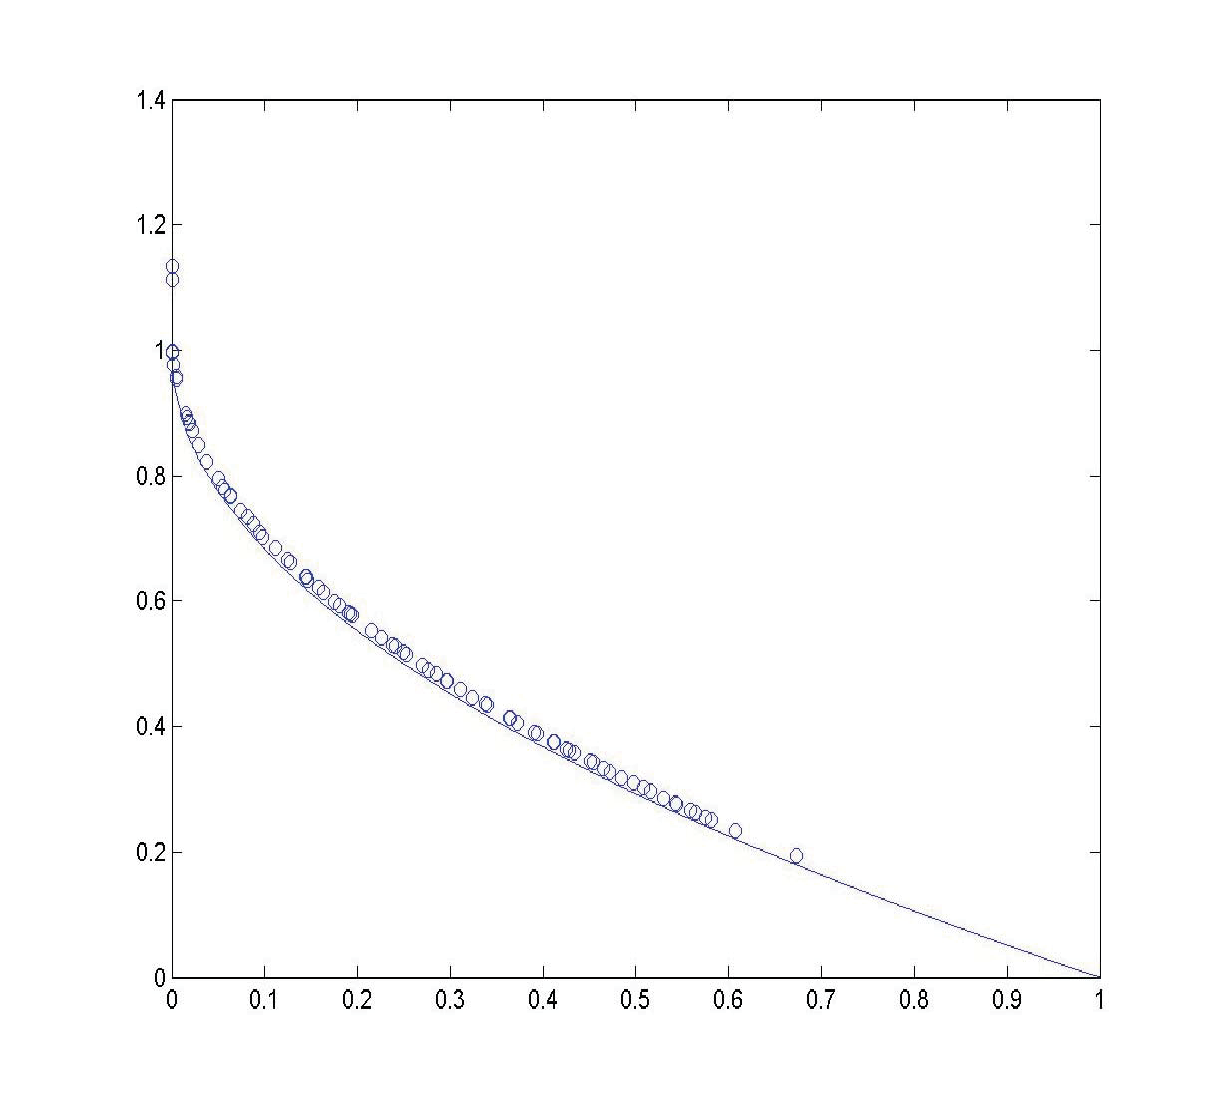
\epsfig{file=./img/metaheuristics/conv-ok-div-fail, width=6.5cm} \\
		(a) & (b) \\
	\end{tabular}
	\caption{Pareto fronts examples with bad convergence (a) and bad diversity (b).} \label{fig:conv.fail.div.ok}
\end{figure}

\subsection{Design aspects}

Adopting techniques based on Pareto optimality within metaheuristic algorithms involves, on the one hand, working with non-dominated solutions that make it necessary to incorporate specific mechanisms to handle them, and on the other hand, to find not a single solution but a set of Pareto-optimal solutions that, besides, must have enough diversity to cover the whole front. Although there are many aspects to consider depending on each specific algorithm, the following ones can be considered common to all of them: fitness function of the solutions, diversity maintenance, and handling constraints. Each one of them is discussed below.

\subsubsection{Fitness function}
\label{sssec:FitnessFunction}

In the running cycle of all metaheuristics, there is always some phase in which the solution that are being handled have to be sorted according to their fitness function in order to select any of them. We refer, for example, to selection and replacement operators in evolutionary algorithms or the updating method of the reference set in scattered search. In the case of single-objective optimization, the fitness of a solution is a unique value and the ordering of solutions is trivial according to this value. However, in our approach to solving MOPs, the fitness is a vector of values (a value for each objective) so ordering is not so straightforward.

\begin{figure}[H] %!t
	\centering
	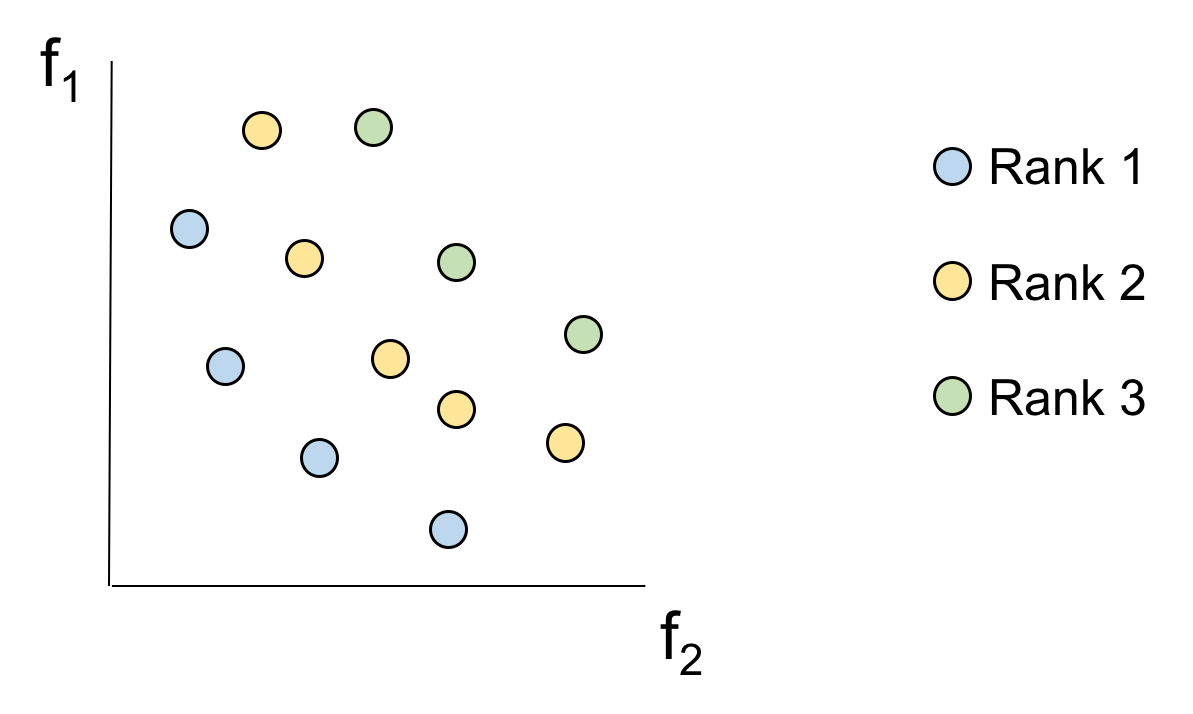
\includegraphics[width=0.60\textwidth]{img/metaheuristics/my-rank.png}
	%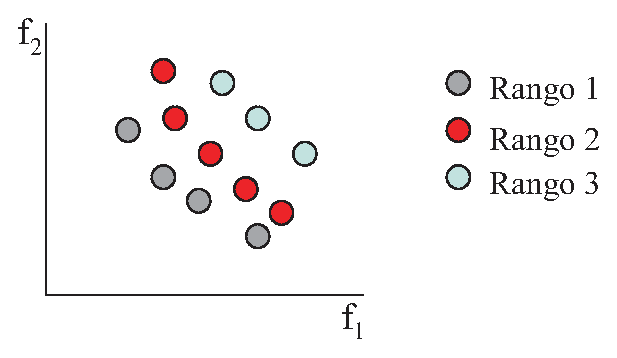
\epsfig{file=./img/metaheuristics/ranking, width=8cm}
	\caption{(\emph{Ranking}) ordering example for solutions in a MOP with two objectives.}
	\label{fig:ranking}
\end{figure}

The dominance relation (Equation~\ref{def:ParetoDominance}) is the key in this type of Pareto optimality-based techniques, since it will allow us to establish a solution ordering. In fact, this relation is a strict partial order relation, since it is not reflexive, neither symmetric, nor antisymmetric, but transitive. Thus, different methods have been proposed in the literature \cite{coello07evolutionary, deb01multiobjective} that basically transform the fitness vector into a unique value using this relation. This strategy was originally proposed by Goldberg in \cite{goldberg89genetic} to guide the population of a GA to the Pareto front of a MOP. The basic idea is to find the solutions of the population that are not dominated by any other. These solutions are assigned the highest order (the best in the ordering established by the dominance relationship). Next, the remaining non-dominated solutions are considered if all previous ones are deleted, to which the next range is assigned. The process continues until all solutions are assigned a range. Figure~\ref{fig:ranking} shows an example of the operation of this sorting method ($f_1$ and $f_2$ are functions to be minimized). This dominance-based ordering is the most basic. Another more advanced, such as \emph{strength} of SPEA2 \cite{zitzler01spea2} also takes into account the number of solutions dominated by each solution.

\subsubsection{Diversity}
\label{sssec:Diversity}

Although the fitness function based on dominance already directs the search towards the Pareto front giving a greater aptitude to the non-dominated solutions, this approximation alone is not sufficient when addressing a MOP. If we remember the Section~\ref{ssec:Objectives}, in addition to converging to the optimal front, the solutions have to be distributed as best as possible on this front in order to offer the expert the widest range of solutions to the multi-objective problem.

\begin{figure}[H] %!ht
	\centering 
	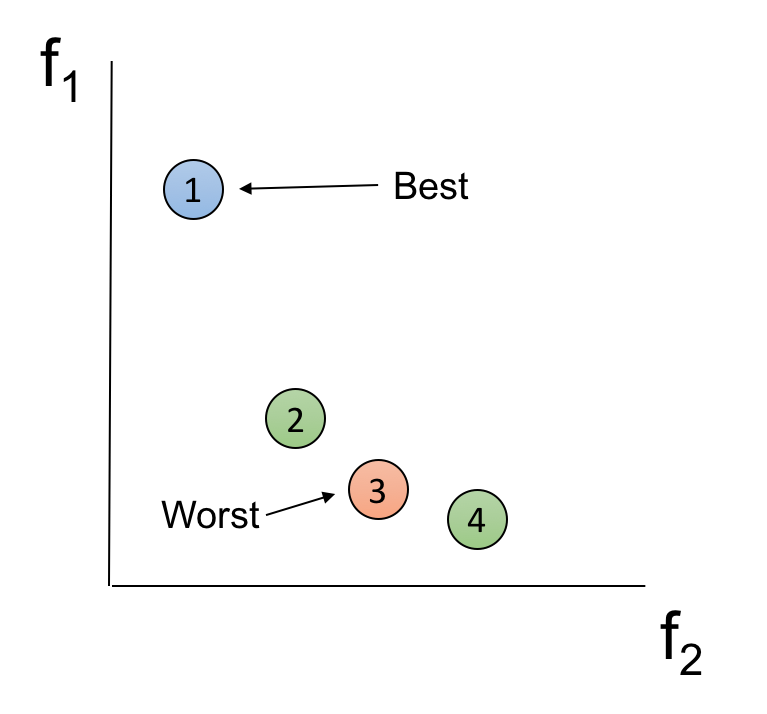
\includegraphics[width=0.40\textwidth]{img/metaheuristics/my-density.png}
	%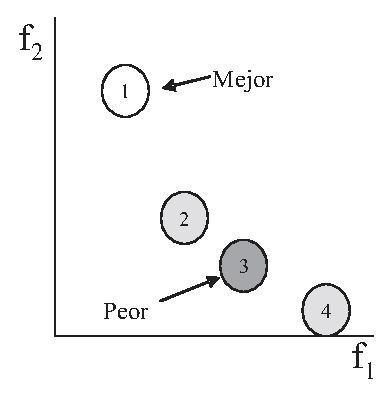
\epsfig{file=./img/metaheuristics/crowding, width=5.5cm}
	\caption{Density estimator example for non-dominated solutions in a MOP with two objectives.}
	\label{fig:crowding}
\end{figure}

Although there are different approaches in the literature \cite{coello07evolutionary}, the most used in the state of the art algorithms are based on complementing the dominance-based fitness function (previous section) with an estimator that measures the density, in the objective space, of solutions around a given solution. Thus, given two solutions with the same fitness (\emph{ranking}, \emph{strength}), the density estimator discriminates between the best and worst solutions taking into account the diversity of them. Let us consider, for example, the set of non-dominated solution in Figure~\ref{fig:crowding}. According to their density, solution 1 can be considered as the best since it is the one that is placed in the less ``populated'' area. Solution 3, on the contrary, would be the worst because it is found in a front area where solutions already exist nearby. Some of the density estimators proposed by the best-known multi-objective algorithms are: \emph{niching} in MOGA \cite{fonseca93multiobjective} and NSGA \cite{srinivas94multiobjective}, the adaptive grid of PAES \cite{KC1999}, \emph{crowding} in NSGA-II \cite{deb02fast} and the distance to the $k$-th neighbor of SPEA2 \cite{zitzler01spea2}.

\subsubsection{Constraint handling} \index{Constraint handling}

The definition of multi-objective problem (Equation~\ref{def:MOP}) included in Section~\ref{ssec:MOBasicConcepts} explicitly includes constraints since, mainly, it is the typical situation when considering real-world problems, as those considered in this thesis. Restrictions can be considered as hard or weak. A constraint is hard when it must be satisfied for a given solution to be acceptable. On the contrary, a weak constraint is one that can be relaxed in some way to accept a solution.

The most used approach in multi-objective metaheuristics of the state-of-the-art to deal with constraints are based on a schema in which feasible solutions are superior to those not feasible \cite{deb00efficient,deb01multiobjective}. That is, given two solutions that are to be compared, three cases can occur:

\begin{enumerate}
	\item If both solutions are feasible, the dominance-based fitness function explained in Section~\ref{sssec:FitnessFunction} is used. In the case in which both solutions are non dominated (equal fitness), a density estimator  (Section~\ref{sssec:Diversity}) is used to discriminate between them.
	
	\item If one solution is feasible and the other is not, the feasible is considered as best.

	\item If both solutions are not feasible, then the one that least violates the constraints is selected.
\end{enumerate}

It remains to be determined how the amount of constraint violation of a given solution is quantified. In order to do this, the most commonly used strategy is to transform all constraints so that they are of type \emph{greater-or-equal-than} zero: $g_i \left (\vec{x}\right) \geq 0$, according to the definition of MOP (Equation~\ref{def:MOP}) \cite{deb01multiobjective}. It can be considered as a type of normalization, so that the value $g_i \left (\vec{x}\right)$ is used to measure how much the constraint is violated. The major drawback to this strategy is given by the equality constraints $h_i\left(\vec{x}\right) = 0$. If it is a weak constraint, it can be relaxed directly to $h_i\left(\vec{x}\right) \geq 0$. However, if $h_i\left(\vec{x}\right) = 0$ is a hard constraint, the transformation is not direct (especially when it is a nonlinear constraint). According to a result obtained in \cite{deb95optimization}, it is possible to convert these hard equality constraints into weak constraints with loss of precision, allowing all constraints of the same type to be already considered. There are many other strategies to deal with constraints in multiobjective optimization \cite{coello07evolutionary, deb01multiobjective} but we have only detailed what will be used in this thesis.

\section{Statistical evaluation of results}
\label{ch.Meta.sec:estadísticas}

As has been commented on several times throughout this document, metaheuristics are non-deterministic techniques. This implies that different runs of the same algorithm on a given problem do not have to find the same solution. This characteristic property of metaheuristics is an important problem for researchers when evaluating their results and, therefore, when comparing their algorithm with other algorithms.

There are some papers that address the theoretical analysis for a large number of heuristics and problems~\cite{graham69bounds, karp77probabilistic}, but given the difficulty of this type of theoretical analysis, the behavior of algorithms is traditionally analyzed by empirical comparisons. For this, it is necessary to define indicators that allow these comparisons. We can find, in general, two different types of indicators. On the one hand, we have those who measure the quality of the solutions obtained. Given that throughout the development of this thesis we have addressed problems of optimization both single- and multi-objective, it is necessary to consider different quality indicators for each type since, although the result in the first case is a single solution (the global optimum), in the second case we have a set of solutions, the optimal Pareto set (Equation~\ref{def:ParetoOptimalSet}). On the other hand, we have the indicators that measure the performance of the algorithms and that refer to the execution times or the amount of computational resources used. We have centered our discussion in the following section in the quality indicators, as the problem executions tackled in this thesis ends at reasonable times, both are closely linked and are often used together for the evaluation of metaheuristics, since the goal of this type of algorithm is to find high quality solutions at a reasonable time.

Once the indicators are defined, a minimum of independent runs of the algorithm must be performed to obtain statistically consistent results.
%A value of 30 is usually considered the minimum acceptable.
A value of 30 is considered a minimum acceptable according to the values often chosen in the literature.
The mere inclusion of means and standard deviations may be insufficient, since erroneous conclusions can be obtained. A global statistical testing may be necessary to assess whether differences are significant and not the
product of random variations~\cite{knowles06tutorial, Garcia2008}. This topic is discussed in more detail in the~\ref{ch.Meta.ssec:analisis} section.

\subsection{Quality indicators}

These indicators are the most important when evaluating a metaheuristic. They are different depending on whether or not the optimal solution of the problem in question is known (a common problem for classical literature, but unusual in real world problems). As already mentioned above, it is necessary to distinguish between indicators for single-objective and multi-objective problems.

\subsubsection{Single-objective optimization indicators}

For instances of problems where the optimal solution is known, it is easy to define an indicator to control the quality of the metaheuristic: the number of times it is reached (\emph {hit rate})\index{Quality indicators!Hit Rate}. This measure is generally defined as the percentage of times the optimal solution is reached with respect to the total number of executions performed. Unfortunately, knowing the optimal solution is not a common case for realistic problems or, even if known, its computation can be so computationally heavy that it is important to find a good approximation in a shorter time. In fact, it is common for experiments with metaheuristics to be limited to performing at most a predefined computational effort (visit a maximum number of points in the search space or a maximum execution time).

In these cases, when the optimum is not known, statistical measures of the corresponding indicator are usually used. The most popular are the average and median of the best fitness value found in each independent run. In general, it is necessary to provide other statistical data such as variance or standard deviation, in addition to the corresponding statistical analysis, to give statistical confidence to the results.

In problems where the optimum is known both metrics can be used, both the number of successes and the average / median of the final (or effort) fitness. What's more, using both gets more information: for example, a low number of hits but a high precision indicates that rarely meets the optimum but is a robust method.

\subsubsection{Multi-objective optimization indicators}

Although the procedure for measuring the quality of solutions in single-objective problems is clear, within the multi-objective field this is a very active research topic~\cite{knowles06tutorial, zitzler03performance}, since the result of these algorithms is a set of non dominated solutions and not a single solution. We must therefore define quality indicators for the Pareto front approaches. There are usually two aspects to consider when measuring the quality of a front: convergence and diversity. The first one refers to the distance between the approach and the optimum Pareto front, while the second measures the uniformity of the solution distribution on the front. As for the single-objective case, there are indicators based on whether or not the optimal front is known.
The quality indicators used in this thesis are Hypervolume ($I_{HV}$)~\cite{zitzler99multiobjective} and Unary Additive Epsilon Indicator ($I_{\epsilon+}$)~\cite{zitzler03performance}, being the two of them Pareto-compliant \cite{knowles06tutorial}. Further details of these indicators are shown below (the interested reader can see~\cite{coello07evolutionary, deb01multiobjective} for other quality indicators defined in the literature):

\begin{itemize}
	
	\item{\bf Hypervolume -- ${\bf I_{HV}}$.}\index{Quality indicator!Hypervolume ($I_{HV}$)} 
	The metric \emph{hypervolume}~\cite{zitzler99multiobjective} is a combined metric of convergence and diversity that calculates the volume, in the objective space, covered by the members of a set $Q$ of non-dominated solutions for the discontinuous line in Figure~\ref{fig:qualityIndicatorHV}, $Q=\{A,B,C\}$) for problems in which all targets must be minimized. Mathematically, for each solution $i\in Q$, a hypercube $v_i$ is constructed using a reference point $W$ (which may be composed of the worst solution for each objective, for example) and the solution $i$ as the corners of the hypercube diagonal. The reference point can be obtained simply by constructing a vector of the worst values for the functions. Thus, $HV$ is calculated as the volume of the union of all hypercubes:
	
	\begin{equation} \label{eq:HV}
	HV = volume\left(\bigcup_{i=1}^{|Q|} v_i \right) \enspace .
	\end{equation}
	
	\begin{figure}[H]
		%\vspace{0.8cm}
		\centering
		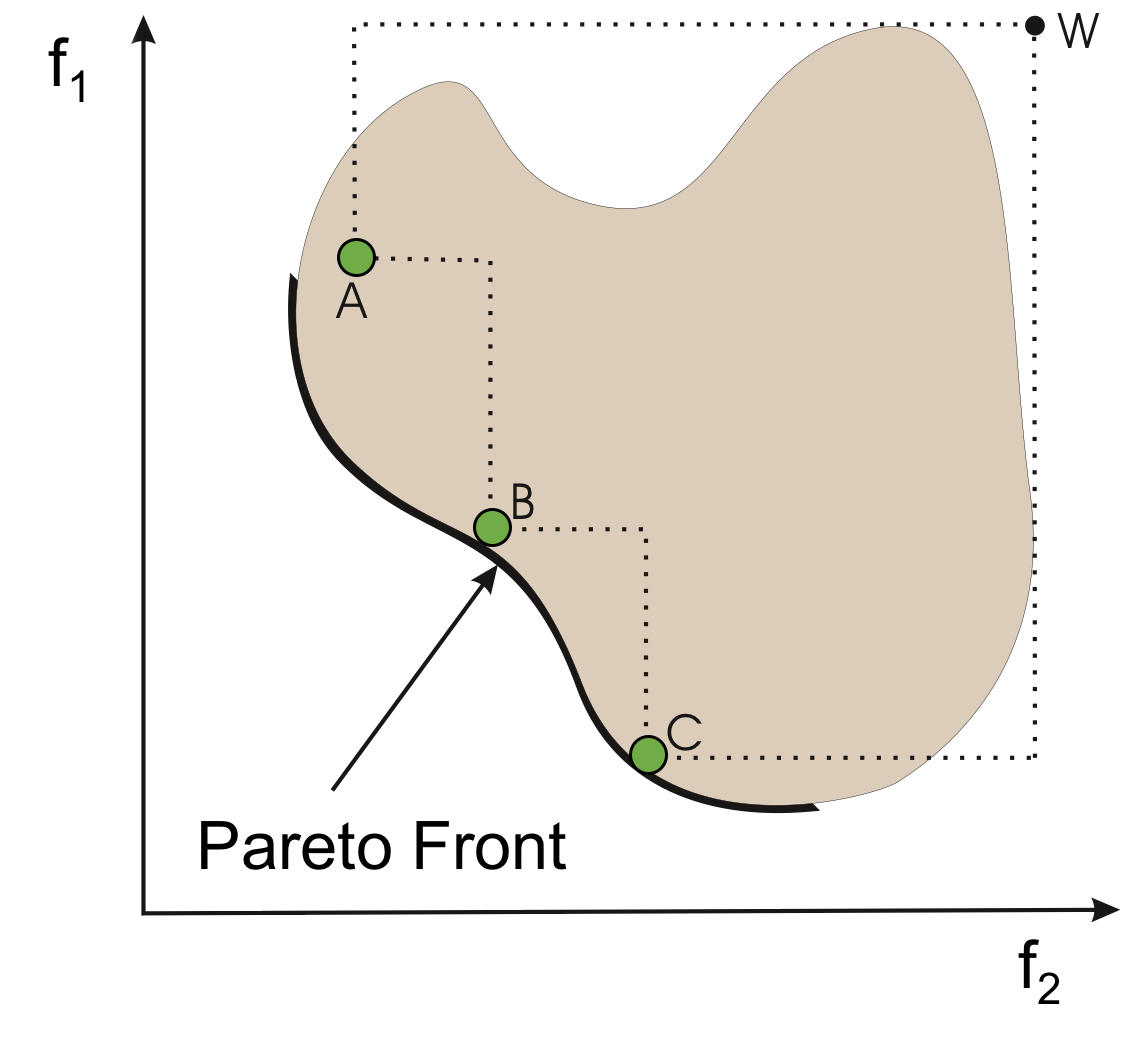
\includegraphics[width=0.50\textwidth]{img/metaheuristics/my-hypervolume.png}
		%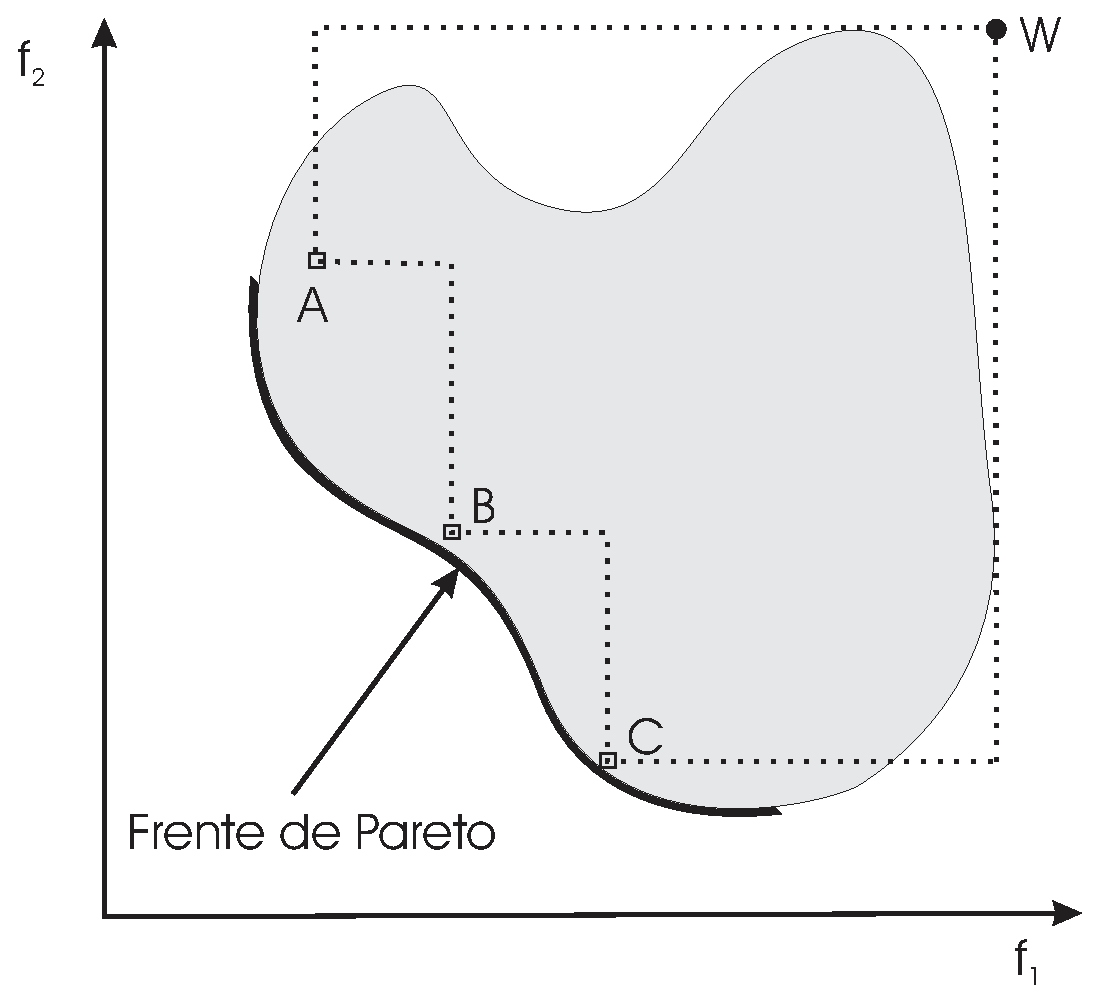
\includegraphics[width=8cm]{./img/metaheuristics/hypervolume}
		%\vspace{0.3cm}
		\caption{Hypervolume covered by the non-dominated solutions.} \label{fig:qualityIndicatorHV}
		% \vspace{0.6cm}
	\end{figure}
	
	\item{\bf Epsilon -- {\bf $I_{\epsilon+}$}.}\index{Quality indicator!Epsilon ($I_{\epsilon+}$)} Given an computed front for a problem, A,
	this indicator is a measure of the smallest distance one would
	need to translate every solution in A so that it dominates the optimal Pareto front
	of this problem~\cite{zitzler03performance}. More formally, given $\vec{z^1} = (z^1_1,\ldots, z^1_n)$ and
	$\vec{z^2} = (z^2_1,\ldots, z^2_n)$, where $n$ is the number of objectives:
	
	\begin{equation}
	I_{\epsilon+}^1(A) = inf_{\epsilon \in \mathbb{R}} \left \{ \forall \vec{z^2} \in \mathcal{PF^*} \;\exists \vec{z^1} \in A: \vec{z^1} \prec_\epsilon 	 \vec{z^2} \right \}
	\end{equation}
	
	\noindent where,
	$ \vec{z^1} \prec_\epsilon \vec{z^2}$ if and only if
	$\forall 1 \leq i \leq n : z^1_i < \epsilon + z^2_i$. In this case, solution fronts with lower values of $I_{\epsilon+}$ are desirable.
	
\end{itemize}


\subsection{Statistical performance assessment}
\label{ch.Meta.ssec:analisis}

As previously explained, metaheuristics are stochastic based algorithms with different random components in their operations. Opposite to deterministic procedures, for which, just a single execution is required, when working with metaheuristics, performing a series of independent runs for each algorithm’s configuration is a mandatory task in order to obtain a distribution of results. In this case, it is possible to compute a global indicator (median, mean, standard deviation, etc.) from the resulted distribution to measure the performance of the studied algorithm. Nevertheless, using one single global indicator to directly compare metaheuristics should lead empirical analyses to biased conclusions. Therefore, the correct practice is to compare the distributions of results by means of statistical tests, which are indispensable tools to validate and to provide confidence to our empirical analysis.

The standard procedure, recommended by the scientific community~\cite{libraco-statistics, Garcia2008}, for the statistical comparison of metaheuristics lies in the use of \emph{parametric} or \emph{non-parametric} tests. Parametric tests show a high precision to detect differences in comparisons, although they are restricted to distributions fulfilling three specific conditions: \emph{independency}, distributions are obtained from independent executions; \emph{normality}, they follow a Gaussian distribution; and \emph{heteroskedasticity}, indicating the existence of a violation of the hypothesis of equality of variances. Non-parametric tests also show a successful performance, although they are less restrictive, since they can be applied regardless of the three previous conditions. Among all these tests, we can find procedures to perform rankings, pair-wise comparisons, and multiple post hoc comparisons.

In this thesis, we have adopted the non-parametric procedure to validate our results and to compare our proposals with other techniques in the current state of the art. Our null hypothesis (equality of distributions) has been set with a confidence level of 95\%, meaning that statistical differences can be found in distributions when resulted tests are with a $p-value < 0.05$. First, \emph{Friedman’s} test is first performed in order to check whether statistical differences exist or not. If so, a \emph{Wilcoxon’s} (signed rank variant) or \emph{Holm’s} tests are performed depending on the number of distributions to compare: 2 or more than 2, respectively. The KEEL (Knowledge Extraction based on Evolutionary Algorithm)~\cite{alcala2011keel} implementation of these tests were used in all the studies that are presented in this thesis.
